\hypertarget{model-implementation-and-replication}{%
\chapter{Model Implementation and
Replication}\label{model-implementation-and-replication}}

Before I extend and experiment on Zollman's, I'll first describe how
exactly I implemented the model in code. While not a traditional part of
most simulation-based modeling papers in philosophy or elsewhere, I
spend time here because I believe better implementations can lead to
better research. Under my view of these sorts of simulations as
experimentally-oriented models, part of the goal of a simulation is to
be easy to experiment on. Because experimentation on a simulation
requires manipulation of that model, a key design goal with this model
was to make modifications as easy as possible. Furthermore, I wanted to
ensure the final result remained performant enough to work well with
large graphs to support modeling the realistic graphs which this project
set out to model.

With that motivation, I adopted the following design goals:

\begin{enumerate}
\def\labelenumi{\arabic{enumi}.}
\tightlist
\item
  Replicate Zollman's specific model correctly.
\item
  Make modifications to model machinery easy and composable.
\item
  Ensure the implementation is fast enough to feasibly run on large
  graphs.
\end{enumerate}

I saw the implementation of this project as an opportunity to push for
more flexible and performant agent-based modeling tools. Most
agent-based modeling tools require models to render to a visual output
on every step and focus on agents which lie on a two-dimensional grid
rather than a rich graph structure. The big names, such as netLogo and
mesa (Python library), both don't do the best job of handling large
models on rich graph structure as a result.

I decided to write my agent-based modeling code from scratch using the
Julia programming language. Julia's combination of multiple-dispatch
support and high performance make it ideal for effective agent-based
modeling for large, heterogeneous systems. While creating a generic
modeling framework was out of the scope of this project, my
implementation of Zollman's models points to an under-served niche:
usable and performance agent-based modeling. Currently, there is little
that falls between graphical interface-based applications like netLogo
or the mesa python library and custom performance-optimized C++
simulations. This means that researchers who build a model can either
use a framework that limits the size and complexity of the models under
study or are forced to spend quite a bit of time crafting custom code
that performs better than the framework.

Julia presents an interesting opportunity here because it is designed
specifically to alleviate this ``two language'' problem where
easy-to-write initial prototype code cannot scale. Thus, I treated my
re-implementation of Zollman's simulation as a trial run to see how the
language did in terms of ease of implementation and simulation
performance. Overall, my experience was positive and has led me to
believe that a more general agent-based modeling framework in Julia
could solve many of the problems in agent-based modeling that I
discussed above.

My implementation of Zollman's model follows directly from its
mathematical structure: it is composed of individuals with beliefs and a
set of global actions that any of the individuals may take. Agents'
actions succeed and fail at the rate set globally and share their
successes and failures with their neighbors.

All of the interactions between agents take place in a step-by-step
fashion where each agent \(A\) does the following at each step:

\begin{enumerate}
\def\labelenumi{\arabic{enumi}.}
\tightlist
\item
  \(A\) chooses one global action to take given \(A\)'s beliefs.
\item
  \(A\) updates \(A\)'s own beliefs according to the number of successes
  and failures from taking the chosen action.
\item
  \(A\) sends its counts of successes and failures to \(A\)'s observers,
  updating their internal beliefs according to their rules.
\end{enumerate}

One interesting note here is that information is transmitted in reverse
as if the author pushed information to observers rather than the
observers stumbling. This leads to much more efficient memory access
patterns by eliminating the need to store the trial counts beyond the
scope of processing a single agent.

Because the processing for any given agent involves sending its
information to its neighbors and updating each neighbor's beliefs, the
running time for any given graph scales proportionally to the number of
edges. The number of edges in a given graph can be very different
between complete graphs, which scale exponentially with the number of
nodes, and cycles which scale linearly. This behavior can be seen in
figures \ref{fig:nbenchmark} and \ref{fig:ebenchmark}, which depicts
benchmark runs which time how long it takes the simulation code to
perform 100 steps.

\begin{figure}
\hypertarget{fig:nbenchmark}{%
\centering
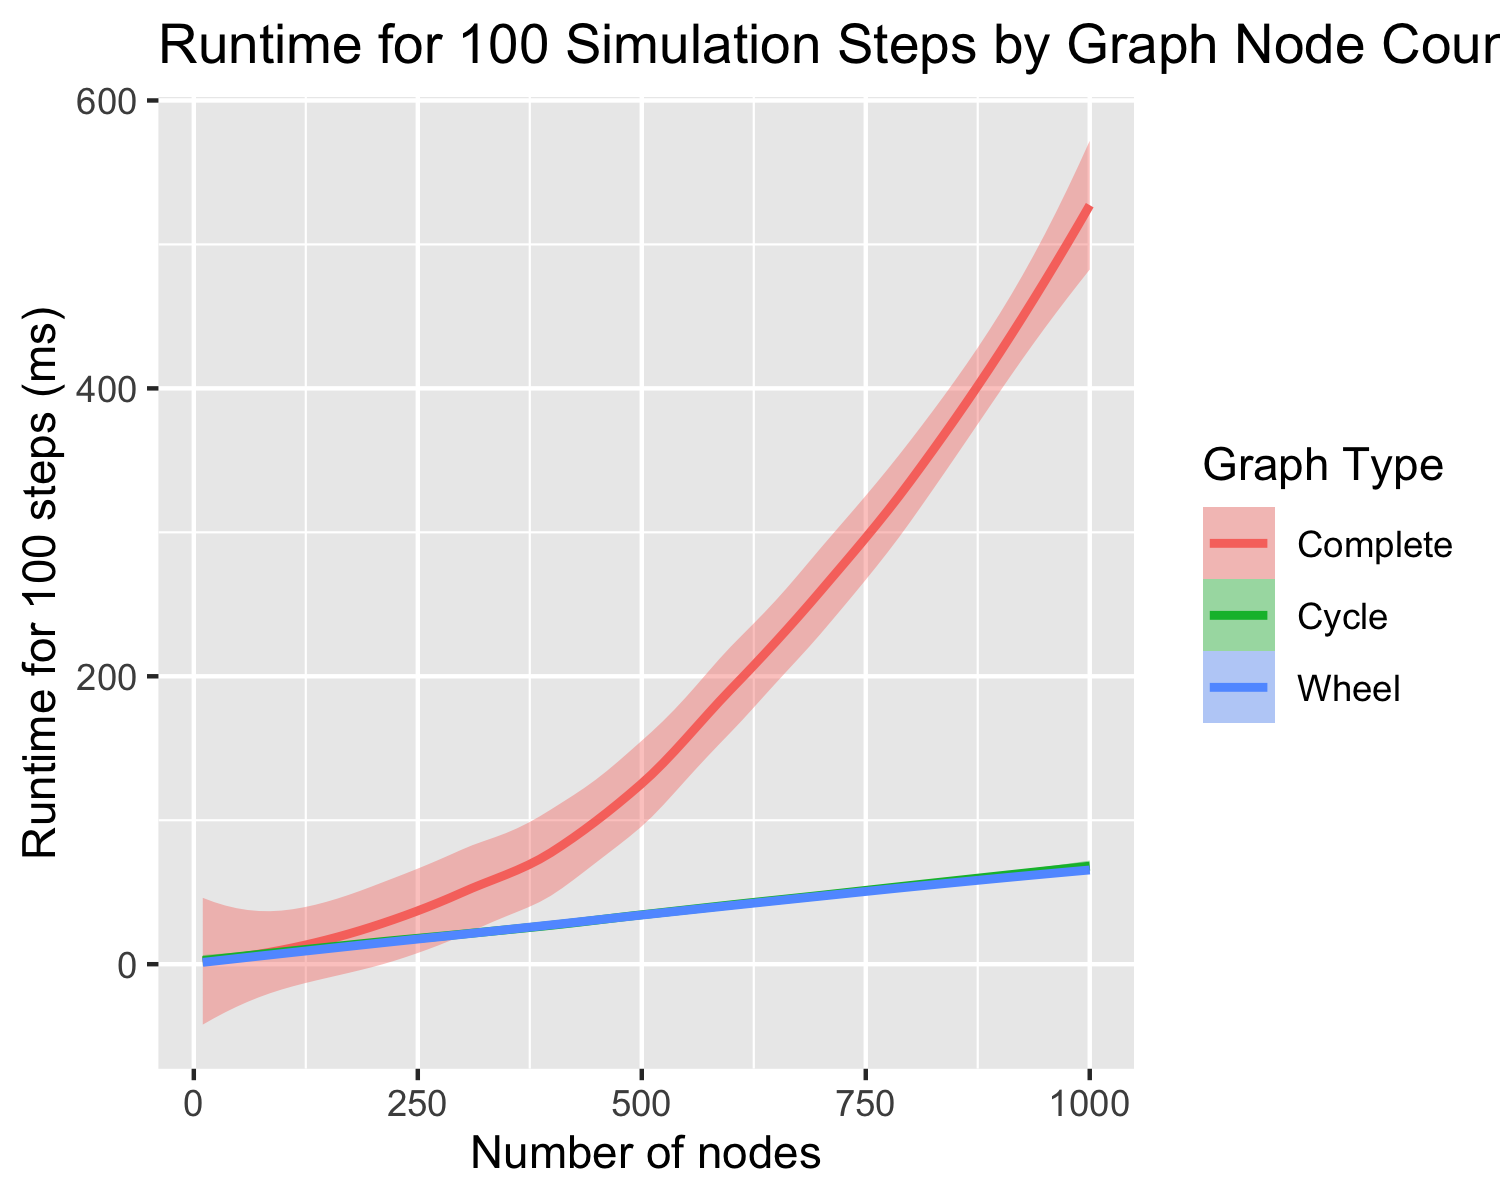
\includegraphics{figures/node_count_benchmarks.png}
\caption{Scaling is not linear in the number of agents (nodes). Note
that complete graphs, which have more edges, take much longer to step
than the wheel and cycle graphs which have fewer edges. The wheel and
cycle graphs take nearly the same time and
overlap.}\label{fig:nbenchmark}
}
\end{figure}

\begin{figure}
\hypertarget{fig:ebenchmark}{%
\centering
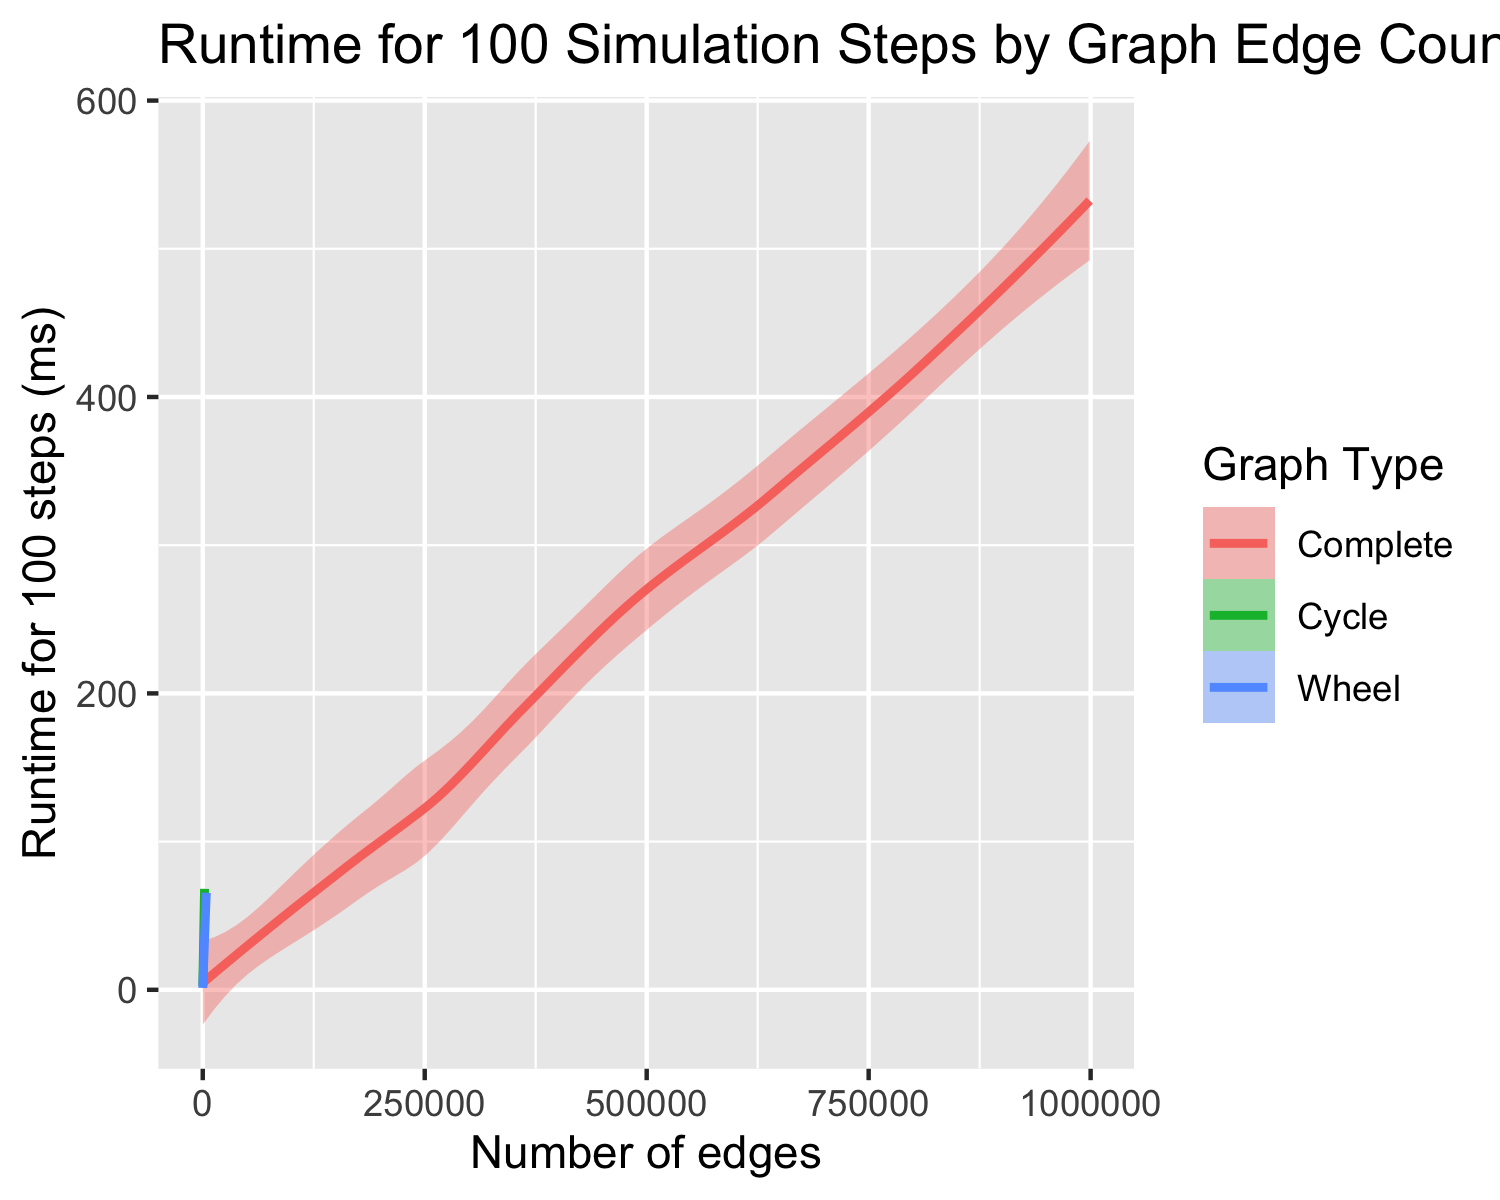
\includegraphics{figures/edge_count_benchmarks.png}
\caption{Scaling is linear in the number of edges as can be seen in the
complete graph scaling line. Note because the complete graph has many
more edges than the wheel and cycle graphs, it is difficult to see the
scaling curves for those graph times on this
graph.}\label{fig:ebenchmark}
}
\end{figure}
